\documentclass[12pt, letterpaper]{article} % [Tamano de la fuente, Tamano del papel]

% Tamano de la pagina y margenes.
\usepackage[letterpaper,top=2cm,bottom=2cm,left=3cm,right=3cm,marginparwidth=1.75cm]{geometry}

% packages utiles
\usepackage{amsmath}
\usepackage[colorlinks=true, allcolors=blue]{hyperref}
\usepackage{graphicx}
\graphicspath{{imagenes\}}} % Direccion de las imagenes
\usepackage{listings}

% Informacion del documento
\title{Trabajo de Investigación - Colecciones en Java}
\author{Equipo 11}
\date{¿? de Octubre de 2022}

% Texto del documento
\begin{document}
\maketitle % Permite la apacion de la informacion del documento

% Nota Negritas: \textbf{greatest}
%      Subrayar: \underline{science} 
%      Cursiva: \textbf{\textit{accident}}

\textbf{Integrantes:}
\begin{itemize}
    \item Alfaro Domínguez Arturo.
    \item Herrera Lezama Fabricio Daniel.
    \item Lopez Gonzalez Erick.
\end{itemize}

\section*{¿Qué son las colecciones?}

Las colecciones representan un grupo de objetos, estos objetos son conocidos como elementos, cuando se necesita trabajar con un conjunto de elementos, se necesita de un contenedor o almacén para guardarlos. En Java se proporciona la interfaz \textbf{Collection}, dicha interfaz permite almacenar cualquier tipo de objeto, como también, es posible usar ciertos métodos para su manipulación, tales como: añadir, eliminar, conocer el tamaño de la colección, etc.
\section*{¿Qué es un marco de recopilación de Java?}

Un marco de recopilación de Java proporciona una arquitectura para almacenar y manipular un grupo de objetos. Un marco de recopilación de Java incluye lo siguiente:

\begin{itemize}
    \item \textbf{Interfaces:} Una interfaz en Java se refiere como tal a los tipos de datos abstractos, permitiendo manipular las colecciones de Java independientemente de los detalles de su representacion. Como tambien, forman una jerarquía en los lenguajes de programación con el paradigma orientado a objetos.
    \item \textbf{Clases:} Las clases para Java son la implementación de la interfaz de colección, es decir, las estructuras de datos que se utilizan.
    \item \textbf{Algoritmo:} Se refiere a los métodos que utilizan para realizar operaciones como búsqueda y clasificación en objetos que se implementan en las interfaces de colección.
    
\end{itemize}

El marco de recopilación de Java proporciona a los desarrolladores el acceso a estructuras de datos pre empaquetadas, así como a algoritmos para manipular datos.

\section*{Modelo de la jerarquía de colecciones en Java}
En el paquete de utilidades de Java (java.util) contiene todas las clases e interfaces que requiere el marco de la colección. El marco de la colección contiene una interfaz denominada interfaz iterable que proporciona el iterador para iterar a través de todas las colecciones. Esta interfaz se amplía con la interfaz de recopilación principal, que actúa como raíz del marco de recopilación. Todas las colecciones amplían esta interfaz de coleccion ampliando así las propiedades del iterador y los métodos de esta interfaz.

A continuación se presenta el diagrama que ilustra la jerarquía de colecciones en Java:
\begin{figure}[h]
    \centering
    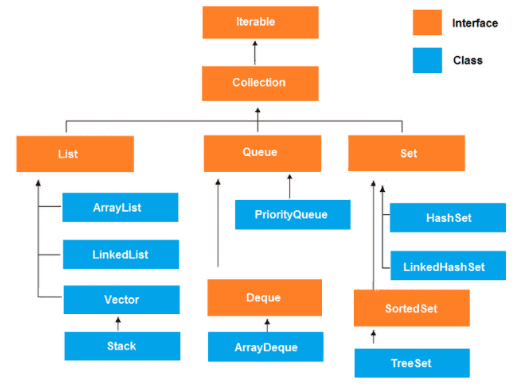
\includegraphics[width=0.75\textwidth]{imagenes/Jerarquia de colecciones Java.png}
    \caption{Jerarquía de Colecciones en Java.}
    \label{fig:jerarquia}
\end{figure}

Con el diagrama presentado, podemos observar cada una de las interfaces y clases que se conforman en dicha jerarquía. Como siguiente se procederá a explicar en detalle  las clases presentadas, sus métodos principales, sus diferencias entre ellas y los aspectos más relevantes al momento de elegir alguno de ellos.

\section{Colecciones de Java: Lista (List)}
Para el apartado de la lista, tenemos que una lista es una colección ordenada de elementos que pueden contener en ellos elementos duplicados. Es una interfaz que amplía la interfaz de colección, dichas listas se clasifican además en lo siguiente:

\begin{enumerate}
    \item \textbf{Lista de arreglo (Array List)}
    \item \textbf{Lista enlazada (Linked List)}
    \item \textbf{Vectores (Vector)}
\end{enumerate}

\section*{- Lista de arreglo (Array List)}
Lista de arreglo o Array List es la implementación de List Interface donde los elementos se pueden agregar o eliminar de forma dinámica en la lista. A su vez, el tamaño de la lista aumenta dinámicamente si los elementos se agregan más que el tamaño que posee en un inicio.

\begin{figure}[h]
    \centering
    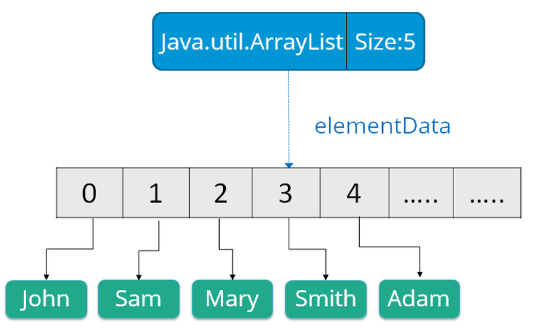
\includegraphics[width=0.75\textwidth]{imagenes/Ejemplo Grafico ArrayList.png}
    \caption{Forma gráfica de la utilería de Java ArrayList.}
    \label{fig:ejemploarraylist}
\end{figure}

\section*{Forma para crear un Array List}
Se debe tomar en cuenta que para su creación se debe importar la biblioteca:

\begin{center}
    import java.util.ArrayList;
\end{center}

A continuación se presenta la forma para declarar un ArrayList:
\begin{center}
    \(ArrayList<[Tipo de dato]> [Identificador] = new ArrayList<[Tipo de dato]>([Tamano]);\)
\end{center}

Donde se tiene que:
\begin{itemize}
    \item \textbf{Tipo de dato:} se definirá el tipo de dato contendra cada uno de los elementos del ArrayList.
    \item \textbf{Identificador:} se definirá su nombre.
    \item \textbf{Tamano:} se le designará el tamaño que tendrá.
\end{itemize}

\section*{Métodos principales en Array List}
\begin{itemize}
    \item \textbf{add():} Añade un elemento a el ArrayList, de forma que este se añade hasta el final. Como parámetro se le da el elemento a insertar.
    
    Ejemplo:
    \lstset{language = Java, breaklines=true, basicstyle=\footnotesize}
    \begin{lstlisting}[frame=single]
    ArrayList<String> al = new ArrayList<String>();
    
    al.add("Luis");
    al.add("Victor");
    al.add("Elena");
    \end{lstlisting}
    
    \item \textbf{remove():} Borra un elemento del ArrayList. Como parámetro se envía el índice del elemento a borrar.
    
    Ejemplo:
    \lstset{language = Java, breaklines=true, basicstyle=\footnotesize}
    \begin{lstlisting}[frame=single]
    ArrayList<String> al = new ArrayList<String>();

    al.add("Victor");    
    al.add("Luis");    
    al.add("Elena");
    
    al.remove(1);
    \end{lstlisting}
    
    \item \textbf{clear():} Limpia el ArrayList de elementos.
    
    Ejemplo:
    \lstset{language = Java, breaklines=true, basicstyle=\footnotesize}
    \begin{lstlisting}[frame=single]
    ArrayList<String> al = new ArrayList<String>();

    al.add("Victor");
    al.add("Luis");
    al.add("Elena");
    al.remove(1);

    al.clear();
    \end{lstlisting}
    
    \item \textbf{size():} Nos devuelve el tamaño o número de elementos del ArrayList.
    
    Ejemplo:
    \lstset{language = Java, breaklines=true, basicstyle=\footnotesize}
    \begin{lstlisting}[frame=single]
    ArrayList<Integer>arrlist = new ArrayList<Integer>();
    
    arrlist.add(1);
    arrlist.add(2);
    arrlist.add(3);
    arrlist.add(4);
    arrlist.add(5);

    System.out.println("Tamano de la lista = " + arrlist.size());
    \end{lstlisting}
    
    \item \textbf{isEmpty():} Verifica si una lista está vacía o no. Devuelve verdadero si la lista no contiene elementos; de lo contrario, devuelve falso si la lista contiene algún elemento.
    
    Ejemplo:
    \lstset{language = Java, breaklines=true, basicstyle=\footnotesize}
    \begin{lstlisting}[frame=single]
    List<Integer> arr = new ArrayList<Integer>(10);
    
    boolean ans = arr.isEmpty();
    
    if(ans == true){
        System.out.println("La lista esta vacia :( ");
    }
    else{
    	System.out.println("La lista no esta vacia :) ");
    }
    \end{lstlisting}

    \item \textbf{indexOf():} Nos devuelve el índice de la primera aparición del elemento especificado en el ArrayList, o -1 si no se contiene el elemento. Como parámetro se envía el elemento a buscar dentro del ArrayList.
    
    Ejemplo:
    \lstset{language = Java, breaklines=true, basicstyle=\footnotesize}
    \begin{lstlisting}[frame=single]
    ArrayList<Integer> arr = new ArrayList<Integer>(5);

    arr.add(1);
    arr.add(2);
    arr.add(3);
    arr.add(4);

    int posicion = arr.indexOf(3);

    System.out.println("El elemento 3 se encuentra en el indice : " + posicion);
    \end{lstlisting}

    \item \textbf{get():} Nos devuelve el elemento en el índice indicado. Como parámetro se le da el índice del elemento que queremos.
    
    Ejemplo:
    \lstset{language = Java, breaklines=true, basicstyle=\footnotesize}
    \begin{lstlisting}[frame=single]
    ArrayList<Integer> lista = new ArrayList<>();

    lista.add(1);
    lista.add(2);
    lista.add(3);

    System.out.println("El primer elemento es: "+ lista.get(0));
    \end{lstlisting}
\end{itemize}

\section*{- Lista enlazada (Linked List)}
La lista vinculada o Linked List, es una secuencia de vínculos que contiene elementos. Cada enlace contiene una conexión a otro enlace.

La clase LinkedList en Java utiliza 2 tipos de listas vinculadas para almacenar los elementos:
\begin{enumerate}
    \item \textbf{Lista individualmente vinculada:} En una lista enlazada individual, cada nodo de esta lista almacena los datos del nodo y un puntero o referencia al siguiente nodo de la lista.
    \begin{figure}[h]
        \centering
        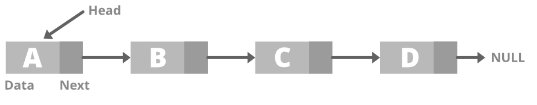
\includegraphics[width=0.75\textwidth]{imagenes/Lista individualmente vinculada.png}
        \caption{Ejemplo gráficdo de una lista individualmente vinculada.}
        \label{fig:individual}
    \end{figure}

    \item \textbf{Lista doblemente enlazada:} En una lista doblemente enlazada, tiene dos referencias, una al nodo siguiente y otra al nodo anterior.
    \begin{figure}[h]
        \centering
        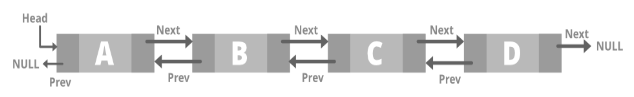
\includegraphics[width=0.75\textwidth]{imagenes/Lista doblemente enlazada.png}
        \caption{Ejemplo gráficdo de una lista doblemente enlazada}
        \label{fig:doblemente}
    \end{figure}

\end{enumerate}

\section*{Forma para crear un LinkedList}
Se debe tomar en cuenta que para su creación se debe importar la biblioteca:

\begin{center}
    import java.util.LinkedList;
\end{center}
A continuación se presenta la forma para declarar un LinkedList:

\begin{center}
    $LinkedList<[Tipo de dato]> [Identificador] = new LinkedList<[Tipo de dato]>([Tamano]);$
\end{center}
Donde se tiene que:
\begin{itemize}
    \item \textbf{Tipo de dato:} Se definirá el tipo de dato contendrá cada uno de los elementos de la LinkedList.
    \item \textbf{Identificador:} Se definirá su nombre.
    \item \textbf{Tamano:} Se le designará el tamaño que tendrá.
\end{itemize}

\section*{Métodos principales en Linked List}
\begin{itemize}
    \item \textbf{add(Objeto):} Nos permite agregar un elemento al final de LinkedList.
    
    \item \textbf{add(int index, Object):} Permite agregar un elemento en un índice en específico en LinkedList.
    
    \lstset{language = Java, breaklines=true, basicstyle=\footnotesize}
    Ejemplo:
    \begin{lstlisting}[frame=single]
    LinkedList<String> LL = new LinkedList<>();

    LL.add("Hola");  
    LL.add(1, "Mundo");
    \end{lstlisting}
    
    \item \textbf{get():} Nos permite buscar o recuperar un elemento de un índice en específico de LinkedList. Como parámetros se le da el índice del elemento que deseamos obtener. Este retorna el elemento encontrado en esa posición.
    
    Ejemplo:
    \lstset{language = Java, breaklines=true, basicstyle=\footnotesize}
    \begin{lstlisting}[frame=single]
    LinkedList<String> list = new LinkedList<String>();

    list.add("Esto");
    list.add(" es");
    list.add(" una prueba");
    list.add(" 10");

    System.out.println("El elemento en la posicion 2 es: "+ list.get(2));
    \end{lstlisting}
    
    \item \textbf{set():} Dado que una LinkedList está indexada, el elemento que deseamos cambiar está referenciado por el índice del elemento. Por lo tanto, este método toma un índice y el elemento actualizado que debe insertarse en ese índice.

    Ejemplo:
    \lstset{language = Java, breaklines=true, basicstyle=\footnotesize}
    \begin{lstlisting}[frame=single]
    LinkedList<String> LL = new LinkedList<>();

    LL.add("Hola");  
    LL.add(1, "Mundo");

    ll.set(1, "a todos");
    \end{lstlisting}
    
    \item \textbf{remove(Object):} Este método se utiliza para eliminar un objeto de LinkedList. De forma que si hay varios objetos de este tipo, se elimina la primera aparición del objeto mandado como parámetro.
    
    \item \textbf{remove(int index):} Dado que una LinkedList está indexada, este método toma un valor entero que simplemente elimina el elemento presente en ese índice específico en LinkedList. Después de eliminar el elemento, todos los elementos se mueven hacia la izquierda para llenar el espacio y se actualizan los índices de los objetos.

    Ejemplo:
    \lstset{language = Java, breaklines=true, basicstyle=\footnotesize}
    \begin{lstlisting}[frame=single]
    LinkedList<String> LL = new LinkedList<>();

    LL.add("Hola");  
    LL.add(" a");
    LL.add(" todos :)");

    LL.remove(1);
    LL.remove(" todos");
    \end{lstlisting}
    
    \item \textbf{contains():} Se utiliza para verificar si un elemento se encuentra dentro de una LinkedList creada. De forma que toma el elemento como parámetro, devuelve verdadero si el elemento se encuentra, en caso contrario, devuelve falso.

    Ejemplo:
    \lstset{language = Java, breaklines=true, basicstyle=\footnotesize}
    \begin{lstlisting}[frame=single]
    LinkedList<String> LL = new LinkedList<>();

    LL.add("Hola");  
    LL.add( " a");
    LL.add( " todos :)");

    if(LL.contains("Hola") == true){
        System.out.println("El elemento 'Hola' se encuentra en la lista :) ");
    }
    else{
    	System.out.println("El elemento no esta en la lista :( ");
    }
    \end{lstlisting}
    
    \item \textbf{peek():} Examina el elemento que se encuentra en el encabezado de la lista, se forma que se recupera mas no se elimina.
    
    \item \textbf{peekFirst():} Similar al método anterior, recupera el primer elemento de esta lista, o devuelve nulo si la lista se encuentra vacía.
    
    \item \textbf{peekLast():} Nos permite recuperar el último elemento que se encuentre en la lista, o devuelve nulo si la lista se encuentra vacía.

    Ejemplo:
    \lstset{language = Java, breaklines=true, basicstyle=\footnotesize}
    \begin{lstlisting}[frame=single]
    LinkedList<String> LL = new LinkedList<>();

    LL.add("Hola");  
    LL.add( " a");
    LL.add( " todos :)");

    System.out.println("Encabezado de la lista: " +LL.peek());

    System.out.println("Primer elemento de la lista: " +LL.peekFirst());

    System.out.println("Ultimo elemento de la lista: " + LL.peekLast());
    \end{lstlisting}

    \item \textbf{clone():} Se utiliza para crear una copia superficial de la lista vinculada. No necesita de un parámetro para su funcionamiento, puesto que solo devuelve una copia de la instancia de la lista.

    Ejemplo:
    \lstset{language = Java, breaklines=true, basicstyle=\footnotesize}
    \begin{lstlisting}[frame=single]
    LinkedList<String> list = new LinkedList<String>();

    list.add("Esto");
    list.add(" es");
    list.add(" una prueba");
    list.add(" 10");

    LinkedList sec_list = new LinkedList();

    sec_list = list.clone();
    \end{lstlisting}
    
\end{itemize}

\section*{- Vectores (Vector):}
Para el caso de los vectores, estos llegan a ser semejantes a las matrices, donde en ellos se puede acceder a los elementos del objeto vectorial, esto por medio de un índice en el vector. Como tal, el vector implementa una matriz dinámica, como también, dicho vector no limita su tamaño.

Si nos damos cuenta, el vector es similar a ArrayList, pero con 2 diferencias:
\begin{enumerate}
    \item El vector está sincronizado.
    \item El vector contiene muchos métodos heredados que no forman parte del marco de las colecciones.
\end{enumerate}

\begin{figure}[h]
    \centering
    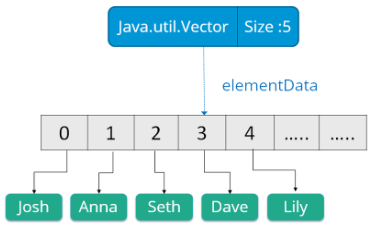
\includegraphics[width=0.75\textwidth]{imagenes/Ejemplo Grafico Vector.png}
    \caption{Ejemplo gráfico de la utilería Java Vector.}
    \label{fig:vector}
\end{figure}

\section*{Forma para crear un Vector}
Se debe tomar en cuenta que para su creación se debe importar la biblioteca:
\begin{center}
    import java.util.Vector;
\end{center}
A continuacion se presenta la forma para declarar un LinkedList:
\begin{center}
    $Vector<[Tipo de dato]> [Identificador] = new Vector<[Tipo de dato]>([Tamano]);$
\end{center}

Donde se tiene que:
\begin{itemize}
    \item \textbf{Tipo de dato:} Se definirá el tipo de dato contendrá cada uno de los elementos del Vector.
    \item \textbf{Identificador:} Se definirá su nombre.
    \item \textbf{Tamano:} Se le designará el tamaño que tendrá.
\end{itemize}

\section*{Métodos principales de Vector}
\begin{itemize}
    \item \textbf{add():} Nos permite añadir un elemento especificado al final de un vector creado, todo esto mediante el aumento del tamaño del vector por 1.

    \item \textbf{add(int index, Object):} El método inserta un elemento en un índice especificado en el vector, de forma que desplaza el elemento que se encuentra actualmente en esa posición, y cualquier elemento posterior a la derecha.

    Ejemplo:
    \lstset{language = Java, breaklines=true, basicstyle=\footnotesize}
    \begin{lstlisting}[frame=single]
    Vector<String> vec_tor = new Vector<String>();

    vec_tor.add("Hola, ");
    vec_tor.add("esto es ");
    vec_tor.add("otra prueba :) ");
    vec_tor.add(1, " . Como estas? ");
    \end{lstlisting}

    \item \textbf{clear():} Se utiliza para eliminar todos los elementos de un vector, es necesario mencionar que el método solo borra los elementos mas no el vector.

    Ejemplo:
    \lstset{language = Java, breaklines=true, basicstyle=\footnotesize}
    \begin{lstlisting}[frame=single]
    Vector<String> vec_tor = new Vector<String>();

    vec_tor.add("Hola, ");
    vec_tor.add("esto es ");
    vec_tor.add("otra prueba :) ");

    vec_tor.clear();

    System.out.println("El vector se encuentra vacio: " + vec_tor);
    \end{lstlisting}

    \item \textbf{remove():} Nos permite eliminar un elemento de un vector mediante una posición o índice dado.

    Ejemplo:
    \lstset{language = Java, breaklines=true, basicstyle=\footnotesize}
    \begin{lstlisting}[frame=single]
    Vector<String> vec_tor = new Vector<String>();

    vec_tor.add("Hola, ");
    vec_tor.add("esto es ");
    vec_tor.add("otra prueba :) ");

    vec_tor.remove(2);
    \end{lstlisting}

    \item \textbf{contains():} Nos permite verificar si un elemento en específico se encuentra en el vector. Como parámetros se le da un elemento del tipo de vector por buscar. Retorna verdadero en caso de encontrar el elemento, caso contrario devuelve falso.

    Ejemplo:
    \lstset{language = Java, breaklines=true, basicstyle=\footnotesize}
    \begin{lstlisting}[frame=single]
    Vector<String> vec_tor = new Vector<String>();

    vec_tor.add("Bienvenidos ");
    vec_tor.add("sean ");
    vec_tor.add("todos ");

    if(vec_tor.contains(":)") == true){
        System.out.println("El elemento esta en el vector :) ");
    }
    else{
	   System.out.println("El elemento no esta en el vector :( ");
    }
    \end{lstlisting}

    \item \textbf{size():} Se utiliza para conocer el tamaño o el número de elementos presentes en el vector. No necesita de un parámetro para su funcionamiento. Retorna el tamaño o la cantidad de elementos en el vector.

    Ejemplo:
    \lstset{language = Java, breaklines=true, basicstyle=\footnotesize}
    \begin{lstlisting}[frame=single]
    Vector<Integer> vec_tor = new Vector<Integer>();

    vec_tor.add(15);
    vec_tor.add(4);
    vec_tor.add(98);
    vec_tor.add(32);

    System.out.println("Tamano del vector:  " + vec_tor.size());
    \end{lstlisting}
    
    \item \textbf{indexOfObject():} Nos permite verificar y encontrar la ocurrencia de un elemento dentro del vector. Como parámetro se envía el elemento del tipo vector. Si el elemento está presente, se devuelve el índice de su primera aparición en el vector, en caso contrario devuelve -1.
    
    Ejemplo:
    \lstset{language = Java, breaklines=true, basicstyle=\footnotesize}
    \begin{lstlisting}[frame=single]
    Vector<Integer> vec_tor = new Vector<Integer>();

    vec_tor.add(15);
    vec_tor.add(4);
    vec_tor.add(98);
    vec_tor.add(32);
    vec_tor.add(4);

    System.out.println("Indice de la primera aparicion del elemento 4: :" + vec_tor.indexOf(4) );
    \end{lstlisting}
\end{itemize}

\section*{- Stack (Pila):}
En el marco de Java Collection, se proporciona la clase Stack (Pila) que modela e implementa una estructura de datos Stack. Un Stack es una estructura de datos lineal que solo tienen un único punto de acceso fijo por el cual se añaden, eliminan o se consultan elementos. El modo de acceso a los elementos es de tipo LIFO ( Last In First Out, último en entrar, primero en salir).

También se puede decir que la clase extiende Vector y trata la clase como una pila, de esta manera, la clase también puede denominarse subclase de Vector.
\section*{Forma para crear un Stack}
Se debe tomar en cuenta que para su creación se debe importar la biblioteca:

\begin{center}
    import java.util.*;
\end{center}

Para este caso en particular donde la clase Stack, se deriva de la clase Vector, se debe realizar lo siguiente:
\begin{center}
    $public class Stack<E> extends Vector<E>$
\end{center}
A continuación se presenta la forma para declarar un Stack:
\begin{center}
    $Stack<[Tipo de dato]> [Identificador] = new Stack<[Tipo de dato]>([Tamano]);$
\end{center}
Donde se tiene que:
\begin{itemize}
    \item \textbf{Tipo de dato:} Se definirá el tipo de dato contendrá cada uno de los elementos del Stack.
    \item \textbf{Identificador:} Se definirá su nombre.
    \item \textbf{Tamano:} Se le designará el tamaño que tendrá.
\end{itemize}

\section*{Métodos principales de Stack}
\begin{itemize}
    \item \textbf{push():} Permite agregar un elemento a la pila, de forma que coloca el elemento en la parte superior de la pila. Como parámetro acepta un elemento de tipo Pila y se refiere al elemento del cual será insertado. 

    Ejemplo:
    \lstset{language = Java, breaklines=true, basicstyle=\footnotesize}
    \begin{lstlisting}[frame=single]
    Stack<String> pila = new Stack<String>();

    pila.push("Hola ");
    pila.push("esto es ");
    pila.push("una prueba :) ");

    System.out.print(pila);
    \end{lstlisting}

    \item \textbf{search():} Permite buscar un elemento dentro de la pila, de tal forma que se obtiene su distancia desde la parte superior. Como parámetro se ingresa el elemento del cual se buscará. El método devuelve la posición del elemento si se encuentra en la pila, en caso de no encontrarlo, se devolverá un -1.

    Ejemplo:
    \lstset{language = Java, breaklines=true, basicstyle=\footnotesize}
    \begin{lstlisting}[frame=single]
    Stack<String> pila = new Stack<String>();

    pila.push("Hola ");
    pila.push("esto es ");
    pila.push("una prueba :) ");

    System.out.println("Posicion del elemento 'Hola': " + pila.search("Hola"));
    \end{lstlisting}

    \item \textbf{pop():} Permite extraer un elemento de la pila. El elemento se saca de la parte superior de la pila y se quita de la misma. El método no necesita de un parámetro para su funcionamiento. De esta forma, devuelve el elemento del cual será quitado, para posteriormente eliminarlo de la pila. 
    
    Ejemplo:
    \lstset{language = Java, breaklines=true, basicstyle=\footnotesize}
    \begin{lstlisting}[frame=single]
    Stack<String> pila = new Stack<String>();

    pila.push("Hola ");
    pila.push("esto es ");
    pila.push("una prueba :) ");

    System.out.println("Se ha quitado el elemento: " + pila.pop());

    System.out.print(pila);
    \end{lstlisting}

    \item \textbf{empty():} Permite verificar si una pila está vacía o no. El método es de tipo booleano y devuelve verdadero si la pila está vacía, de lo contrario, devolverá falso.

    Ejemplo:
    \lstset{language = Java, breaklines=true, basicstyle=\footnotesize}
    \begin{lstlisting}[frame=single]
    Stack<String> pila = new Stack<String>();

    System.out.println("La pila se encuentra vacia? " + pila.empty());
    \end{lstlisting}
\end{itemize}

\section{Colecciones de Java: Cola (Queue)}
En Java, la estructura de Cola ordena los elementos de la manera FIFO (First In, First Out ó Primero en entrar, Primero en salir). En la Cola, el primer elemento ingresado se elimina primero, y el último se elimina al final.

Los métodos básicos de la Cola existe de 2 formas:v
\begin{enumerate}
    \item Se lanza una excepción si se falla la operación.
    \item Devuelve un valor especial.
\end{enumerate}
\begin{figure}[h]
    \centering
    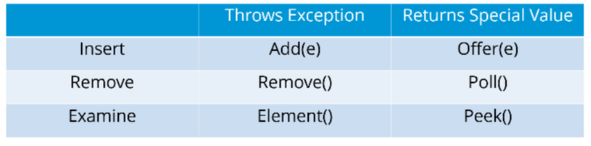
\includegraphics[width=0.75\textwidth]{imagenes/Metodos basicos de la Cola .png}
    \caption{Pie de pagina.}
    \label{fig:tabla}
\end{figure}
Para este caso en cuestión, la cola prioridad se implementa en la interfaz de Cola, de esta manera, cada elemento se ordena de acuerdo con su orden natural, o por un comparador proporcionado en el momento de la construcción de la cola.

\section*{Forma para crear un Queue}
Se debe tomar en cuenta que para su creación se debe importar la biblioteca:
\begin{center}
    import java.util.Queue;
\end{center}
A continuación se presenta la forma para declarar un LinkedList:
\begin{center}
    $Queue<[Tipo de dato]> [Identificador] = new Queue<[Tipo de dato]>([Tamano]);$
\end{center}
Donde se tiene que:
\begin{itemize}
    \item \textbf{Tipo de dato:} Se definirá el tipo de dato contendrá cada uno de los elementos del Queue.
    \item \textbf{Identificador:} Se definirá su nombre.
    \item \textbf{Tamano:} Se le designará el tamaño que tendrá.
\end{itemize}

\section*{Métodos principales de Cola (Queue)}
\begin{itemize}
    \item \textbf{add():} Inserta un elemento pasado en el parámetro al final de la cola en caso de haber espacio. Si la cola al momento de insertar un elemento se encuentra en su capacidad límite, devolverá una excepción.
    
    Ejemplo:
    \lstset{language = Java, breaklines=true, basicstyle=\footnotesize}
    \begin{lstlisting}[frame=single]
    Queue<Integer> cola = new LinkedList<Integer>();

    cola.add(444);
    cola.add(356);
    cola.add(890);

    System.out.println("Cola: " + cola);
    \end{lstlisting}

    \item \textbf{offer():} Permite insertar un el elemento especificado en la cola si es posible hacerlo inmediatamente sin violar las restricciones de su capacidad. Este método es preferible al método add(), ya que este método no lanza una excepción cuando la capacidad del contenedor está llena, puesto que solo devuelve un falso.
    
    Ejemplo:
    \lstset{language = Java, breaklines=true, basicstyle=\footnotesize}
    \begin{lstlisting}[frame=single]
    Queue<Integer> cola = new LinkedList<Integer>(3);

    cola.add(444);
    cola.add(356);
    cola.add(890);

    if(cola.offer(250)){
        System.out.println("Se ha insertado el elemento 250 en la cola :) ");
    }
    else{
    	System.out.println("La cola se encuentra llena :( ");
    }
    \end{lstlisting}

    \item \textbf{remove():} Devuelve y elimina el elemento al frente de la cola. El método regresa una excepción en caso de que la cola esté vacía.
    
    Ejemplo:
    \lstset{language = Java, breaklines=true, basicstyle=\footnotesize}
    \begin{lstlisting}[frame=single]
    Queue<Integer> cola = new LinkedList<Integer>();

    cola.add(444);
    cola.add(356);
    cola.add(890);
    cola.add(777);

    System.out.println("Elemento eliminado de la cabeza de la cola: " + cola.remove());
    \end{lstlisting}

    \item \textbf{poll():} Similar al método anterior, devuelve y elimina el elemento al frente de la cola. La diferencia de este método respecto a remove(), se debe a que este no lanza una excepción cuando la cola está vacía, en su lugar devuelve un valor nulo.
    
    Ejemplo:
    \lstset{language = Java, breaklines=true, basicstyle=\footnotesize}
    \begin{lstlisting}[frame=single]
    Queue<Integer> cola = new LinkedList<Integer>();

    cola.add(444);
    cola.add(356);
    cola.add(890);
    cola.add(777);

    System.out.println("Elemento eliminado de la cabeza de la cola: " + cola.poll());
    \end{lstlisting}

    \item \textbf{element():} Devuelve el elemento que se encuentre al frente de la cola, es necesario mencionar que dicho elemento no lo elimina. Su funcionamiento es semejante a peek(), pero su diferencia radica en que solo lanza una excepción si la cola está vacía.
    
    Ejemplo:
    \lstset{language = Java, breaklines=true, basicstyle=\footnotesize}
    \begin{lstlisting}[frame=single]
    Queue<Integer> cola = new LinkedList<Integer>();

    cola.add(444);
    cola.add(356);
    cola.add(890);
    cola.add(777);
    
    System.out.println("Elemento en la cabeza de la cola: " + cola.element());
    \end{lstlisting}
\end{itemize}

\section{Colecciones de Java: Conjuntos (Sets)}
Un conjunto se refiere a una colección que no puede contener elementos duplicados. Su uso se enfoca principalmente en modelar la abstracción de conjuntos matemáticos. Para este caso Set tiene su implementación en varias clases como:
\begin{enumerate}
    \item \textbf{Hashsests}
    \item \textbf{LinkedHashet}
    \item \textbf{TreeSet}
\end{enumerate}

\section*{- HashSet}
En Java, la clase HashSet crea una colección que usa una tabla hash para su almacenamiento. HashSet solo puede contener elementos únicos, a su vez, hereda la clase AbstractSet e implementa la interfaz Set.

\section*{Forma para crear un HashSet}
Se debe tomar en cuenta que para su creación se debe importar la biblioteca:
\begin{center}
    import java.util.HashSet;
\end{center}
A continuación se presenta la forma para declarar un HashSet:
\begin{center}
   $HashSet<[Tipo de dato]> [Identificador] = new HashSet<[Tipo de dato]>([Tamano]);$ 
\end{center}
Donde se tiene que:
\begin{itemize}
    \item \textbf{Tipo de dato:} Se definirá el tipo de dato contendrá cada uno de los elementos del HashSet.
    \item \textbf{Identificador:} Se definirá su nombre.
    \item \textbf{Tamano:} Se le designará el tamaño que tendrá.
\end{itemize}

\section*{Métodos principales de Hashset}
\begin{itemize}
    \item \textbf{add():} Permite añadir o insertar elementos al Hashset, sin embargo, la orden de inserción no se conserva. Es necesario tener en cuenta que los elementos duplicados no están permitidos, por lo que cada elemento duplicado que se encuentre se ignorará.

    Ejemplo:
    \lstset{language = Java, breaklines=true, basicstyle=\footnotesize}
    \begin{lstlisting}[frame=single]
    HashSet<String> hs = new HashSet<String>();

    hs.add("A");
    hs.add("B");
    hs.add("C");
    hs.add("D");
    \end{lstlisting}

    \item \textbf{contains():} Verifica si un elemento específico se encuentra dentro del HashSet. Como parámetro se envía un elemento del tipo HashSet. Retorna  verdadero si el elemento se encuentra, en caso contrario devuelve falso.

    Ejemplo:
    \lstset{language = Java, breaklines=true, basicstyle=\footnotesize}
    \begin{lstlisting}[frame=single]
    HashSet<String> hs = new HashSet<String>();

    hs.add("A");
    hs.add("B");
    hs.add("C");
    hs.add("D");

    if(hs.contains("D") == true){
        System.out.println("La letra 'D' esta presente :) ");
    }
    else{
	   System.out.println("La letra 'D' no esta :( ");
    }
    \end{lstlisting}

    \item \textbf{clear():} Permite eliminar todos los elementos de un HashSet. El uso de este método solo borra todos los elementos del conjunto, mas no elimina al conjunto.

    Ejemplo:
    \lstset{language = Java, breaklines=true, basicstyle=\footnotesize}
    \begin{lstlisting}[frame=single]
    HashSet<String> hs = new HashSet<String>();

    hs.add("A");
    hs.add("B");
    hs.add("C");
    hs.add("D");

    System.out.println("Conjunto despues de usar clear(): " + hs.clear());
    \end{lstlisting}

    \item \textbf{isEmpty():} Permite verificar si un Hashset se encuentra vacío. Este devuelve verdadero si el HashSet está vacío, en caso contrario devolverá un falso.

    Ejemplo:
    \lstset{language = Java, breaklines=true, basicstyle=\footnotesize}
    \begin{lstlisting}[frame=single]
    HashSet<String> hs = new HashSet<String>();

    hs.add("A");
    hs.add("B");
    hs.add("C");
    hs.add("D");

    if(hs.isEmpty() == true){
        System.out.println("El conjunto esta vacio :) ");
    }
    else{
    	System.out.println("El conjunto tiene elementos :( ");
    }
    \end{lstlisting}

    \item \textbf{remove():} Permite eliminar un elemento especificado dentro del HashSet.

    Ejemplo:
    \lstset{language = Java, breaklines=true, basicstyle=\footnotesize}
    \begin{lstlisting}[frame=single]
    HashSet<String> hs = new HashSet<String>();

    hs.add("A");
    hs.add("B");
    hs.add("C");
    hs.add("D");

    hs.remove("D");
    \end{lstlisting}

    \item \textbf{clone():} Se utiliza para devolver una copia superficial del conjunto de hash. No necesita de ningún parámetro para su funcionamiento.

    Ejemplo:
    \lstset{language = Java, breaklines=true, basicstyle=\footnotesize}
    \begin{lstlisting}[frame=single]
    HashSet<Integer> hs = new HashSet<Integer>();

    hs.add(1);
    hs.add(2);
    hs.add(3);
    hs.add(4);

    HashSet hs_2  = new HashSet();

    hs_2 = hs.clone();

    System.out.println("Nuevo conjunto clonado: " + hs_2);
    \end{lstlisting}

    \item \textbf{size():} Permite obtener el tamaño, o conocer la cantidad de elementos que se encuentran en el HashSet.

    Ejemplo:
    \lstset{language = Java, breaklines=true, basicstyle=\footnotesize}
    \begin{lstlisting}[frame=single]
    HashSet<Integer> hs = new HashSet<Integer>();

    hs.add(1);
    hs.add(2);
    hs.add(3);
    hs.add(4);

    System.out.println("Tamano del conjunto: " + hs.size());
    \end{lstlisting}
\end{itemize}

\section*{- LinkedHashSet (HashSet vinculado)}
En Java, HashSet vinculado o LinkedHashSet es una tabla Hash con una implementación de lista vinculada de la interfaz Set.
Contiene elementos únicos como HashSet, también, proporciona cada uno de los métodos HashSet, manteniendo el orden de inserción.

\section*{Forma para crear un LinkedHashSet}
Se debe tomar en cuenta que para su creación se debe importar la biblioteca:
\begin{center}
    import java.util.LinkedHashSet;
\end{center}
A continuación se presenta la forma para declarar un LinkedHashSet:
\begin{center}
    $LinkedHashSet<[Tipo de dato]> [Identificador] = new LinkedHashSet<[Tipo de dato]>([Tamano]);$
\end{center}
Donde se tiene que:
\begin{itemize}
    \item \textbf{Tipo de dato:} Se definirá el tipo de dato contendrá cada uno de los elementos del LinkedHashSet.
    \item \textbf{Identificador:} Se definirá su nombre.
    \item \textbf{Tamano:} Se le designará el tamaño que tendrá.
\end{itemize}

\section*{- TreeSet}
La clase TreeSet implementa la interfaz Set, del cual usa un árbol binario para su almacenamiento. Cada uno de los objetos se almacenan en orden ascendente. Dicha clase hereda la clase AbstractSet e implementa la interfaz NavigableSet. Al igual que las anteriores clases, este solo puede contener elementos únicos. La clase TreeSet llega a ser mucho más rápida en el tiempo de acceso y recuperación de los elementos.

\section*{Forma para crear un TreeSet}
Se debe tomar en cuenta que para su creación se debe importar la biblioteca:
\begin{center}
    import java.util.Set;
\end{center}
A continuación se presenta la forma para declarar un TreeSet:
\begin{center}
    $Set<[Tipo de dato]> [Identificador] = new TreeSet<[Tipo de dato]>([Tamano]);$
\end{center}
Donde se tiene que:
\begin{itemize}
    \item \textbf{Tipo de dato:} Se definirá el tipo de dato contendrá cada uno de los elementos del TreeSet.
    \item \textbf{Identificador:} Se definirá su nombre.
    \item \textbf{Tamano:}  Se le designará el tamaño que tendrá.
\end{itemize}

\section*{Métodos principales de TreeSet}
\begin{itemize}
    \item \textbf{add():} Permite agregar un elemento en específico dentro de un TreeSet. El método agrega al elemento sólo si el elemento no se encuentra, caso contrario el método devuelve un falso.
    
    \item \textbf{addAll():} Permite agregar todos los elementos de la colección al conjunto creado. Cada uno de los elementos se agregan aleatoriamente sin seguir ningún orden específico.
    
    Ejemplo:
    \lstset{language = Java, breaklines=true, basicstyle=\footnotesize}
    \begin{lstlisting}[frame=single]
    TreeSet<String> tree = new TreeSet<String>();

    tree.add("Hola ");
    tree.add("esto es ");
    tree.add("una prueba ");

    TreeSet<String> tree_2 = new TreeSet<String>();

    tree_2.add("Bienvenidos ");
    tree_2.add("sean todos ");

    tree.addAll(tree_2);

    System.out.println("TreeSet: " + tree);
    \end{lstlisting}

    \item \textbf{contains():} Se utiliza para comprobar si un elemento específico está presente en el TreeSet. Devuelve verdadero si el elemento se encuentra dentro del TreeSet, en caso contrario devuelve un falso.

    \item \textbf{containsAll():} Permite comprobar si dos conjuntos contienen los mismos elementos o no. Toma un conjunto como parámetro y devuelve verdadero si todos los elementos de este conjunto están presentes en el otro conjunto
    
    Ejemplo:
    \lstset{language = Java, breaklines=true, basicstyle=\footnotesize}
    \begin{lstlisting}[frame=single]
    TreeSet<Integer> set = new TreeSet<Integer>();

    set.add(12);
    set.add(99);
    set.add(42);
    set.add(30);

    System.out.println("El conjunto contiene al 99? "+ set.contains(99));

    TreeSet<Integer> set_2 = new TreeSet<Integer>();

    set_2.add(12);
    set_2.add(99);
    set_2.add(42);
    set_2.add(30);

    System.out.println("El conjunto 1 contiene al conjunto 2?  " +  set.containsAll(set_2));
    \end{lstlisting}

    \item \textbf{isEmpty():} Permite comprobar y verificar si un TreeSet se encuentra vacío. Retorna verdadero si el TreeSet está vacío, en caso contrario devuelve falso.
    
    Ejemplo:
    \lstset{language = Java, breaklines=true, basicstyle=\footnotesize}
    \begin{lstlisting}[frame=single]
    TreeSet<String> tree = new TreeSet<String>();

    if(tree.isEmpty() == true){
        System.out.println("El conjunto esta vacio :) ");
    }
    else{
	   System.out.println("El conjunto tiene elementos :( ");
    }
    \end{lstlisting}

    \item \textbf{remove():} Permite eliminar un elemento en particular de un TreeSet. Como parámetros se le da el elemento del cual se eliminará del conjunto. Retorna verdadero si se elimina el elemento dado del conjunto, de lo contrario devuelve falso.
    
    Ejemplo:
    \lstset{language = Java, breaklines=true, basicstyle=\footnotesize}
    \begin{lstlisting}[frame=single]
    TreeSet<Integer> set = new TreeSet<Integer>();

    set.add(12);
    set.add(99);
    set.add(42);
    set.add(30);

    sett.remove(42);

    System.out.println("Nuevo conjunto despues de haber eliminado el elemento 42: " + set);
    \end{lstlisting}

    \item \textbf{clear():} Permite eliminar todos los elementos de un TreeSet. Al usar este método borra únicamente los elementos del conjunto, mas no el conjunto.

    Ejemplo:
    \lstset{language = Java, breaklines=true, basicstyle=\footnotesize}
    \begin{lstlisting}[frame=single]
    TreeSet<Integer> set = new TreeSet<Integer>();

    set.add(12);
    set.add(99);
    set.add(42);
    set.add(30);

    set.clear();

    System.out.println("Conjunto despues haber eliminado sus elementos: " + set);
    \end{lstlisting}

    \item \textbf{clone():} Devuelve una copia superficial del conjunto de arboles.

    Ejemplo:
    \lstset{language = Java, breaklines=true, basicstyle=\footnotesize}
    \begin{lstlisting}[frame=single]
    TreeSet<String> tree = new TreeSet<String>();

    tree.add("Hola ");
    tree.add("esto es ");
    tree.add("una prueba ");

    TreeSet tree_2 = new TreeSet();

    tree_2 = tree.clone();

    System.out.println("Conjunto clonado: " + tree_2);
    \end{lstlisting}

    \item \textbf{fist():} Permite devolver el primero de los elementos de un TreeSet. El primer elemento aquí se refiere al más bajo de los elementos del conjunto, puesto que nos encontramos en un conjunto de árboles. Es necesario mencionar que si los elementos son de tipo entero, se devuelve el número entero más pequeño; en caso de ser elementos de tipo string, los elementos se verifican en orden alfabético.

    \item \textbf{last():} Permite devolver el último elemento de un TreeSet. El último elemento aquí se refiere al más alto de los elementos del conjunto. Es necesario mencionar que si los elementos son de tipo entero, se devuelve el entero más grande; en caso de ser elementos de tipo string, los elementos se verifican en orden alfabético

    Ejemplo:
    \lstset{language = Java, breaklines=true, basicstyle=\footnotesize}
    \begin{lstlisting}[frame=single]
    TreeSet<Integer> tree = new TreeSet<Integer>();

    tree.add(500);
    tree.add(12);
    tree.add(210);
    tree.add(98);
    tree.add(7);

    System.out.println("El primer elemento del conjunto es: " + tree.first());

    System.out.println("El ultimo elemento del conjunto es: " + tree.last());
    \end{lstlisting}

    \item \textbf{size():} Nos permite obtener el tamaño del conjunto de árboles, o la cantidad de elementos presentes en él. No necesita de un parámetro para su funcionamiento.

    Ejemplo:
    \lstset{language = Java, breaklines=true, basicstyle=\footnotesize}
    \begin{lstlisting}[frame=single]
    TreeSet<Integer> tree = new TreeSet<Integer>();

    tree.add(500);
    tree.add(12);
    tree.add(210);
    tree.add(98);
    tree.add(7);

    System.out.println("Tamano del conjunto: " + tree.size());
    \end{lstlisting}
\end{itemize}

\section*{+ Interfaz de Mapa}
La interfaz Mapa no pertenece como un subtipo de la interfaz de Colección. Como tal la interfaz Map, representa un mapeo entre una clave y un valor. Por lo tanto, esta se comporta distinta al resto de tipos de colecciones de Java. Es necesario mencionar que un mapa solo contiene claves únicas.

\begin{figure}[h]
    \centering
    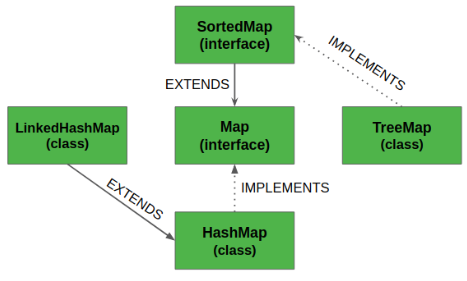
\includegraphics[width=0.75\textwidth]{imagenes/Interfaz de Mapa.png}
    \caption{Relación de la interfaz de Mapas con las colecciones de Java.}
    \label{fig:IMapa}
\end{figure}

\section*{Forma para crear un HashMap}
Se debe tomar en cuenta que para su creación se debe importar la biblioteca:
\begin{center}
    import java.util.HashMap;
\end{center}
A continuación se presenta la forma para declarar un Map

\begin{center}
    $Map<[Clave][Valor]> [Identificador] = new HashMap<[Tipo de dato]>([Tamano]);$
\end{center}
Donde se tiene que:
\begin{itemize}
    \item \textbf{Clave:} El tipo de clave que tendrá el mapa.
    \item \textbf{Valor:}  El tipo de valores mapeados.
    \item \textbf{Tamaño:} Se le designará el tamaño que tendrá.
    \item \textbf{Identificador:} Se definirá su nombre.
\end{itemize}

\section*{Métodos principales de HashMap}

\begin{itemize}
    \item \textbf{put():} Permite asociar un valor especificado con una clave del mapa. Como parámetros, se requiere de 2 argumentos (clave y valor), donde la clave es el primer argumento ingresado, y el segundo argumento es el valor correspondiente de la clave en el mapa. A su vez, el método devuelve el valor anterior asociado con la clave si esta se encuentra presente, en caso de no serlo, devolverá un -1.
    
    Ejemplo:
    \lstset{language = Java, breaklines=true, basicstyle=\footnotesize}
    \begin{lstlisting}[frame=single]
    Map<Integer, String> map = new HashMap<>();

    map.put(1, "Uno");
    map.put(2, "Dos");
    map.put(3, "Tres");

    System.out.println(map);
    \end{lstlisting}

    \item \textbf{remove():} Permite eliminar el mapeo de una clave. Como argumento, se le asigna la clave del argumento, del cual se procederá a eliminar. 
    
    Ejemplo:
    \lstset{language = Java, breaklines=true, basicstyle=\footnotesize}
    \begin{lstlisting}[frame=single]
    Map<Integer, String> map = new HashMap<>();

    map.put(1, "Uno");
    map.put(2, "Dos");
    map.put(3, "Tres");

    map.remove(2);

    System.out.println(map);
    \end{lstlisting}

    \item \textbf{containsKey():} Permite verificar si una clave en particular se encuentra mapeado, de forma que toma el elemento de la clave como parámetro y devuelve verdadero si ese elemento está mapeado, en caso contrario devolverá un falso.
    
    Ejemplo:
    \lstset{language = Java, breaklines=true, basicstyle=\footnotesize}
    \begin{lstlisting}[frame=single]
    Map<Integer, String> map = new HashMap<>();

    map.put(12, "Hola");
    map.put(24, "Esto es");
    map.put(31, "una prueba");

    System.out.println("Se encuentra la clave 24? "+map.containsKey(24));
    \end{lstlisting}

    \item \textbf{clear():} Permite eliminar todos los elementos de una colección de mapas.
    
    Ejemplo:
    \lstset{language = Java, breaklines=true, basicstyle=\footnotesize}
    \begin{lstlisting}[frame=single]
    Map<Integer, String> map = new HashMap<>();

    map.put(12, "Hola");
    map.put(24, "Esto es");
    map.put(31, "una prueba");

    map.clear();

    System.out.println(map);
    \end{lstlisting}

    \item \textbf{hashCode():} Permite generar un código hash para el mapa dado de claves y valores. No necesita de argumentos para su funcionamiento. El método devuelve el valor HashCode para el mapa especificado.

    Ejemplo:
    \lstset{language = Java, breaklines=true, basicstyle=\footnotesize}
    \begin{lstlisting}[frame=single]
    Map<Integer, String> map = new HashMap<>();

    map.put(12, "Hola");
    map.put(24, "Esto es");
    map.put(31, "una prueba");
    map.put(7, ":D");

    int hash = map.hashCode();

    System.out.println("Codigo Hash del mapa: "+hash);
    \end{lstlisting}

    \item \textbf{entrySet():} Permite crear un conjunto de los mismos elementos del mapa especificado. No necesita de parámetros para su funcionamiento. El método devuelve un conjunto que tiene los mismos elementos que el mapa especificado. 
    
    Ejemplo:
    \lstset{language = Java, breaklines=true, basicstyle=\footnotesize}
    \begin{lstlisting}[frame=single]
    Map<Integer, String> map = new HashMap<>();

    map.put(12, "Hola");
    map.put(24, "Esto es");
    map.put(31, "una prueba");
    map.put(7, ":D");

    System.out.println(map.entrySet());
    \end{lstlisting}

    \item \textbf{equals():} Permite verificar la igualdad entre 2 mapas, de forma que verifica si los elementos de un mapa pasados como parámetro son iguales a los elementos del mapa especificado. Como parámetro, se ingresa el objeto de tipo mapa del cual se verifica la igualdad. El método devuelve verdadero si la igualdad existe entre ambos mapas, en caso contrario devolverá un falso.
    
    Ejemplo:
    \lstset{language = Java, breaklines=true, basicstyle=\footnotesize}
    \begin{lstlisting}[frame=single]
    Map<Integer, String> map_1 = new HashMap<>();
    Map<Integer, String> map_2 = new HashMap<>();

    map_1.put(12, "Hola");
    map_1.put(24, "Esto es");
    map_1.put(31, "una prueba");
    map_1.put(7, ":D");

    map_2.put(1, "Uno");
    map_2.put(2, "Dos");
    map_2.put(3, "Tres");

    System.out.println("El mapa 1 es igual al mapa 2? "+map_1.equals(map_2));
    \end{lstlisting}
\end{itemize}

\section*{Referencias electronicas:}
\begin{itemize}
    \item ArrayList en Java – Acervo Lima. (s. f.). Recuperado 24 de septiembre de 2022, de \href{https://bit.ly/3fB4HAN}{https://es.acervolima.com/arraylist-en-java/}
    
    \item Clase de vector en Java – Acervo Lima. (s. f.). Recuperado 24 de septiembre de 2022, de \href{https://es.acervolima.com/clase-de-vector-en-java-1/}{https://es.acervolima.com/clase-de-vector-en-java-1/}
    
    \item COLECCIONES JAVA: INTERFAZ, LISTA, COLA, CONJUNTOS EN JAVA CON EJEMPLOS - BLOG. (s. f.). Recuperado 24 de septiembre de 2022, de \href{https://es.quish.tv/java-collections-interface}{https://es.quish.tv/java-collections-interface}
    
    \item Interfaz de mapa en Java – Acervo Lima. (s. f.). Recuperado 30 de septiembre de 2022, de \href{https://es.acervolima.com/interfaz-de-mapa-en-java/}{https://es.acervolima.com/interfaz-de-mapa-en-java/}
    
    \item Interfaz de cola en Java – Acervo Lima. (s. f.). Recuperado 24 de septiembre de 2022, de \href{https://es.acervolima.com/interfaz-de-cola-en-java/}{https://es.acervolima.com/interfaz-de-cola-en-java/}
    
    \item LinkedList en Java – Acervo Lima. (s. f.). Recuperado 24 de septiembre de 2022, de \href{https://es.acervolima.com/linkedlist-en-java-1/}{https://es.acervolima.com/linkedlist-en-java-1/}
\end{itemize}

\end{document}